\documentclass[12pt]{article}
\usepackage[utf8]{inputenc}
\usepackage[T1,T2A]{fontenc}
\usepackage{hyperref}
\hypersetup{colorlinks=true, linkcolor=blue, filecolor=magenta, urlcolor=cyan}
\urlstyle{same}
\usepackage{amsmath}
\usepackage{amsfonts}
\usepackage{amssymb}
\usepackage[version=4]{mhchem}
\usepackage{stmaryrd}
\usepackage{bbold}
\usepackage{graphicx}
\usepackage[export]{adjustbox}
\usepackage{mathtools}
\usepackage{makecell}
\usepackage{parskip}
\usepackage{geometry}
\usepackage{fancyhdr}
\usepackage{float}

\geometry{margin=1in}

\graphicspath{ {notes-02-dropout-batchnorm} }

\pagestyle{fancy}
\fancyhf{}
\lhead{Глубинное обучение 1, 2025/26}
\rhead{ФКН ВШЭ}
\cfoot{\thepage}
\renewcommand{\headrulewidth}{0.5pt}

\newcommand{\verteq}{\rotatebox{90}{$\,=$}}
\newcommand{\equalto}[2]{\underset{\scriptstyle\overset{\mkern4mu\verteq}{#2}}{#1}}
\makeatletter
\newcommand{\course}[1]{\gdef\@course{#1}}
\gdef\@course{}
\renewcommand{\maketitle}{%
  \begin{center}
    {\Large\textbf{\@title}}\\[0.3cm]
    {\Large\textbf{\@course}}\\[0.2cm]
    {\large\@author}\\[0.2cm]
    {\normalsize\@date}
  \end{center}
  \vspace{0.3cm}
  \noindent\rule{\textwidth}{0.5pt}
  \vspace{0.5cm}
}
\makeatother
\title{ФКН ВШЭ}
\course{Глубинное обучение 1, 2025/26}
\author{Автор конспекта: Архипов Виктор}
\date{25 марта 2026 г.}

\begin{document}
\thispagestyle{empty}
\maketitle




\makeatletter
\renewcommand{\tableofcontents}{%
  \section*{\contentsname}
  {\large
  \@starttoc{toc}%
  }
}
\makeatother
\tableofcontents
\newpage
\begin{center}
\setcounter{section}{1}
\section*{Lecture 2: NLLLoss, Dropout and Batch Norm}
\addcontentsline{toc}{section}{Лекция 2: NLLLoss, Dropout and Batch Norm}
\vspace{0.3cm}
\noindent\rule{\textwidth}{0.5pt}
\end{center}

\subsection{Classification}
Minimize error rate:
$$\frac{1}{l} \sum_{i=1}^{l} \mathbb{1}[\alpha(x_i) \neq y_i]$$

where:
\begin{itemize}
  \item $l$ — number of samples
  \item $\alpha(x_i) = \hat{y_i}$ — predicted label
  \item $y_i$ — true label, $y_i \in \{1, \ldots, c\}$
  \item $\mathbb{1}[\cdot]$ — indicator function
\end{itemize}
\textbf{Problem:} This loss function is \textbf{discrete} and non-differentiable. It provides \textbf{no meaningful gradient signal} for backpropagation through deeper layers. The indicator function $\mathbb{1}[\cdot]$ returns only 0 or 1, with a derivative of zero almost everywhere. This makes standard gradient-based optimization impossible.

\textbf{Solution:} We need a continuous, differentiable loss function (for example cross-entropy) that provides useful gradients for training deep neural networks.

$$p = \begin{pmatrix}
p(\hat{y}_i = 1) \\
p(\hat{y}_i = 2) \\
\vdots \\
p(\hat{y}_i = c)
\end{pmatrix}$$

$$z_i = \sigma(W_i z_{i-1} + b_i)$$

$$z_n \in \mathbb{R}^c, \quad z_n = W_n z_{n-1} + b_n, \quad W_n \in \mathbb{R}^{d_{n-1} \times c}$$

$$p = \{p_i\}_{i=1}^{c}, \quad p_i \geq 0, \quad \sum_{i=1}^{c} p_i = 1$$
To ensure these conditions are satisfied, we must apply the softmax function to $z_n$:

$$\text{Softmax}: p_i = \frac{e^{z_i}}{\sum_{j=1}^{c} e^{z_j}}, \quad z_i - \text{logits}$$
Since softmax is monotonic in its input, 
$z_i > z_j \implies p_i > p_j$


As we can see, it guarantees that $p_i \geq 0$ and $\sum_{i=1}^{c} p_i = 1$.

\subsection{Negative Log Likelihood (NLL)}

For a target class $y \in \{1, \ldots, c\}$, the loss function is:

$$L = -\sum_{k=1}^{c} \mathbb{1}[k = y] \log p_k = -\log p_y \longrightarrow \min$$

where:
\begin{itemize}
  \item $y$ — true class label
  \item $p_k$ — predicted probability for class $k$
  \item $\mathbb{1}[k = y]$ — indicator function (1 if $k = y$, 0 otherwise)
\end{itemize}

% This can be rewritten as:
% $$-\sum_{k=1}^{c} \log p_{y_i} \longrightarrow\min$$
For a training set $\{(x_i, y_i)\}_{i=1}^{l}$, where $y_i \in \{1, \ldots, c\}$ target:
% \mathcal{L}(x_i, y_i) =
$$ -\sum_{i=1}^{\ell} \sum_{k=1}^{c} \mathbb{1}[k = y_i] \log p_k^{(i)} \longrightarrow \min_{W,b} $$

Equivalently:
$$-\sum_{i=1}^{\ell} \log p_{y_i}^{(i)} \longrightarrow \min_{W,b} \iff \prod_{i=1}^{\ell} p_{y_i}^{(i)} \longrightarrow \max$$
In terms of probability as $Softmax(z_i)$: 
$$\text{NLLLoss}(\text{Softmax}(z), y) \longrightarrow \min$$
This idea comes from mathematical statistics. We want to maximize the probability assigned to the true class, which is equivalent to minimizing the negative log likelihood.

However this formula is not numerically stable for computations without trick. Thus:

$$\log \text{softmax}(z_i) = \log \frac{\exp(z_i)}{\sum_{j=1}^{c} \exp(z_j)} = \log \exp(z_i) - \log \left(\sum_{j=1}^{c} \exp(z_j)\right)$$

$$= z_i - \log \sum_{j=1}^{c} \exp(z_j) = z_i - \text{logsumexp}$$

where:
\begin{itemize}
  \item $z_i$ — raw logit for class $i$
  \item $\log \sum_{j=1}^{c} \exp(z_j)$ — log-sum-exp (numerically stable)
\end{itemize}

To improve numerical stability, we use:
$$\log \frac{\exp(z_i - \max_j z_j)}{\sum_{j=1}^{c} \exp(z_j - \max_j z_j)}$$

This prevents overflow/underflow by subtracting the maximum logit before exponentiation (e.g. IEEE 754).

Implementation in torch is CrossEntropyLoss, during inference, softmax converts logits to probabilities:
$$\text{CE}(\{p_i\}_{i=1}^{c}, \{q_i\}_{i=1}^{c}) = -\sum_{i=1}^{c} q_i \log p_i, \quad q_i = \mathbb{1}[i=y] $$

where:
\begin{itemize}
  \item $\{p_i\}$ — predicted probabilities (from softmax)
  \item $\{q_i\}$ — true class distribution (one-hot encoded)
\end{itemize}




% \subsection{Regularization}
\subsection{Label Smoothing, Blending}
As we showed before $q_i$ assigns probability 1 to the true class and 0 to all others:
$$q_i = \begin{cases} 1 & \text{if } i = y \\ 0 & \text{otherwise} \end{cases}$$

However, this can lead to overconfidence and poor generalization. Label smoothing introduces a small uniform probability to all classes:

$$q_i = \begin{cases} 1 - \frac{c-1}{c}\epsilon & \text{if } i = y \\ \frac{\epsilon}{c} & \text{otherwise} \end{cases}$$

where $\epsilon$ is the smoothing parameter (typically $\epsilon = 0.1$).

% Example with $c = 10$ classes and $\epsilon = 0.1$:

% \begin{itemize}
%   \item True class $y$: $q_y = 1 - \frac{9}{10} \cdot 0.1 = 1 - 0.09 = 0.91$
%   \item All other classes: $q_i = \frac{0.1}{10} = 0.01$ (for $i \neq y$)
% \end{itemize}

% Alternatively, this can be written as:
% $$q_i = (1 - \epsilon) \cdot \mathbb{1}[i = y] + \frac{\epsilon}{c}$$
This method acts as a regularization technique and improves generalization to unseen data.

\textbf{Blending}

Blending combines two objects (e.g., images) with a fixed weight:
$$x_{\text{blend}} = \alpha x_1 + (1 - \alpha) x_2$$

where $\alpha \in [0, 1]$ is a fixed blending coefficient (e.g., $\alpha = 0.5$).

The target is also blended:
$$y_{\text{blend}} = \alpha y_1 + (1 - \alpha) y_2$$

This creates a soft target that reflects both classes in the mixed image.

% \textbf{Mixup:}
% Mixup extends blending by randomly sampling $\lambda \sim \text{Beta}(\alpha, \alpha)$ for each training sample, and randomly pairing examples within a batch. 
% $$x_{\text{mix}} = \lambda x_1 + (1 - \lambda) x_2$$
% $$y_{\text{mix}} = \lambda y_1 + (1 - \lambda) y_2$$

\subsection{Dropout}

Dropout is a regularization technique that randomly removes neurons during training to prevent overfitting.

 $z_k \in \mathbb{R}^{B \times d_k}$ where: $B$ — batch size, $d_k$ — hidden dimension (number of neurons)

\textbf{Train mode:}

We sample a binary matrix $m \in  \{0,1 \}^{B \times d_k}$, where $m_{ij} \sim \text{Bernoulli}(1 - p)$ for each activation:
$$y = \text{dropout}(z_k) = m \odot z_k$$
$$\mathbb{E}[y_i] = \mathbb{E}[m_i \odot z_k^{(i)}] = \mathbb{E}[m_i]\odot z_k^{(i)} = (1-p) z_k^{(i)} $$
To maintain the expected value of activations, we need to scale by $\frac{1}{1-p}$ due to the fact $\mathbb{E}[m_{ij}] = 1-p$:
$$y = \text{dropout}(z_k) = \frac{m}{1-p} \odot z_k$$

This ensures that $\mathbb{E}[y] = \mathbb{E}[z_k]$ during training.

\textbf{Eval mode:}

No dropout is applied and all neurons are used.
$$y_{\text{inference}} = z$$

Or equivalently, use inverted dropout during training (scale by $\frac{1}{1-p}$) and no scaling at inference.

\textbf{Why Dropout works:}
Forces the network to learn redundant representations and acts as ensemble of many thinned networks

\begin{figure}[H]
  \centering
  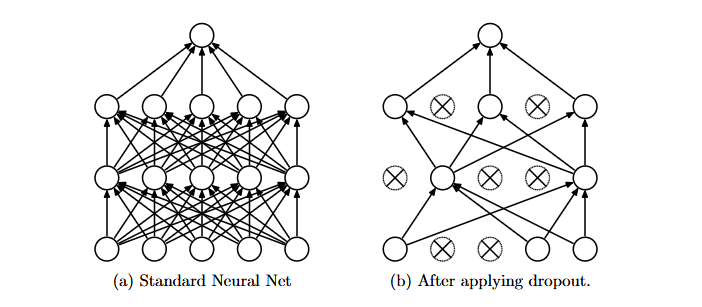
\includegraphics[width=0.7\textwidth]{Screenshot_4.png}
  \caption{Adapted from Srivastava, Nitish, et al. "Dropout: a simple way to prevent neural networks from overfitting", JMLR 2014}
  \label{fig:dropout}
\end{figure}

\subsection{Batch Normalization}

Batch Normalization normalizes the inputs to each layer, which stabilizes and accelerates training.


\textbf{Train mode:}

$z_i \in \mathbb{R}^{B \times d}$ where: $B$ — batch size, $d$ — feature dimension

Computation of batch statistics
$$\mu = \frac{1}{B} \sum_{i=1}^{B} z_i, \quad \sigma^2 = \frac{1}{B} \sum_{i=1}^{B} (z_i - \mu)^2$$
$$\hat{z}_i = \frac{z_i - \mu}{\sqrt{\sigma^2 + \epsilon}}$$

where $\epsilon$ is a small constant for numerical stability.

$$y_i = \hat{z_i}\odot w + b$$

where $w,b \in \mathbb{R}^{d_k}$ are trainable by gradient descent.

\textbf{Eval mode}
On inference we usually process data differently from batches. That is why instead of using batch statistics, we use running statistics computed during training on every batch:
$\mu, \sigma $ - collect statistics over all training batches. 
$$running\_mean_m  := running\_mean_{m-1}\cdot(1-\gamma) + \mu_m\cdot \gamma$$
$$\text{running\_var}_m := \text{running\_var}_{m-1} \cdot (1-\gamma) + \sigma^2_m \cdot \gamma \frac{B}{B-1} \quad \text{(unbiased)}$$


$$\hat{z}_i = \frac{z_i - {\text{running\_mean}}}{\sqrt{{\text{running\_var}} + \epsilon}}$$
$$y_i = \hat{z_i}\odot w + b$$

\textbf{Benefits of Batch Normalization:}

Batch Normalization reduces internal covariate shift, which allows the network to use higher 
learning rates without becoming unstable. It makes training faster and more stable by ensuring 
that the distribution of inputs to each layer remains consistent throughout training.
\end{document}
